\documentclass[12pt,compress,english,utf8,t]{beamer}

\usepackage{etex}

\usepackage[english]{babel}

\usepackage{tikz}
\usepackage{booktabs}
\usepackage{ragged2e}

\usetikzlibrary{calc,shapes.callouts,shapes.arrows}
\definecolor{darkred}{RGB}{220,0,0}
\newcommand{\hcancel}[5]{%
    \tikz[baseline=(tocancel.base)]{
        \node[inner sep=0pt,outer sep=0pt] (tocancel) {#1};
        \draw[darkred, line width=1mm] ($(tocancel.south west)+(#2,#3)$) -- ($(tocancel.north east)+(#4,#5)$);
    }%
}%

\usepackage[protrusion=true,expansion=true]{microtype}

\title{The secret of the number 5}
\author{Ingo Blechschmidt}
\institute{32th Chaos Communication Congress}
\date{December 28th, 2015}

\usetheme{Warsaw}
\usecolortheme{seahorse}
\definecolor{mypurple}{RGB}{60,0,255}
\setbeamercolor{structure}{fg=mypurple}
\usefonttheme{serif}
\usepackage[T1]{fontenc}
\usepackage{libertine}
\useinnertheme{rectangles}
\setbeamercovered{invisible}

\setbeamertemplate{title page}[default][colsep=-1bp,rounded=false,shadow=false]
\setbeamertemplate{frametitle}[default][colsep=-2bp,rounded=false,shadow=false,center]

\setbeamertemplate{navigation symbols}{}
\setbeamertemplate{headline}{}

\newcommand*\oldmacro{}%
\let\oldmacro\insertshorttitle%
\renewcommand*\insertshorttitle{%
  \oldmacro\hfill\insertframenumber\,/\,\inserttotalframenumber\hfill}

\newcommand{\hil}[1]{{\usebeamercolor[fg]{item}{\textbf{#1}}}}

\newcommand{\atpos}[1]{%
  \begin{tikzpicture}[remember picture, overlay]%
    \node[anchor=south east] at (current page.south east) {#1};
  \end{tikzpicture}%
}

\newcommand{\centeredpar}[2]{%
  \begin{center}
    \colorbox{white}{\parbox{#1\textwidth}{%
      #2%
    }}%
  \end{center}%
}

\newcommand{\sourcedquote}[4]{%
  ``#1''\par%
  {\raggedleft -- #2, #3, \href{#4}{\underline{link}}\par}%
}

% Gonzalo Medina, http://tex.stackexchange.com/a/228198
\makeatletter
\def\Mdescription#1{%
  \advance\beamer@descdefault by \labelsep%
  \list
  {}
  {\labelwidth\beamer@descdefault%
  \leftmargin\beamer@descdefault%
  \let\makelabel\beamer@descriptionitem
  \settowidth\labelwidth{\beamer@descriptionitem{#1}}%
  \setlength\leftmargin{\labelwidth}% 
  \addtolength\leftmargin{\labelsep}%
  }%
  \beamer@cramped%
  \raggedright
  \beamer@firstlineitemizeunskip%
}
\def\endMdescription{\ifhmode\unskip\fi\endlist}
\long\def\beamer@descriptionitem#1{%
  \def\insertdescriptionitem{#1}%
  {\usebeamertemplate**{description item}}\hfil}
\makeatother

\setbeameroption{show notes}
\setbeamertemplate{note page}[plain]

\begin{document}

\frame{
  \titlepage

  \vspace*{-2em}
  \begin{center}
    \small
    \emph{Watch this space for details on the talk.}
    \medskip

    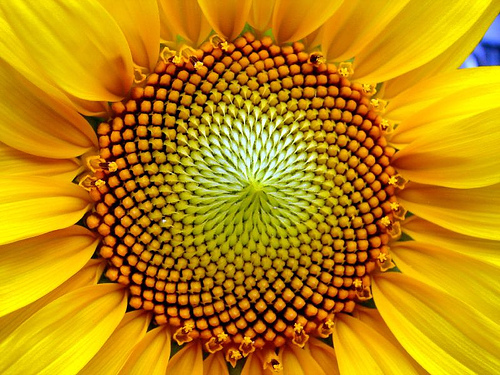
\includegraphics[height=0.25\textheight]{sonnenblume}\quad
    
\includegraphics[height=0.25\textheight]{mandelbrot}\quad
    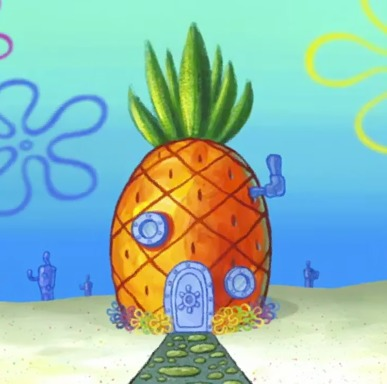
\includegraphics[height=0.25\textheight]{spongebob-ananas}
  \end{center}
}

% http://joachim-reichel.org/software/fraktal/mandelbrot_large.png

\end{document}

Plan of the talk:

1. Images of spirals in nature; notice Fibonacci numbers.
2. Infinite continued fraction:
   * Example with [1; 2, ...]
   * More examples (only listed)
   * Euclidean algorithm (with illustration?)
   * Theorem about best approximation
3. Approximation of pi
   * List original sources for 22/7 and 355/113
   * Explain using continued fractions
4. Spirals in nature
   * angle, need "most irrational number"
   * golden ratio (also explain as a ratio)
   * simulations
5. Fibonacci numbers in the Mandelbrot fractal
6. Vi Hart
